% Chapter 4 opener diagram: "Plots of Multivariate Data"
% Center bubble = chapter; satellites = its numbered sections.
% Section list mirrors the chapter .qmd — update here when sections change,
% then rebuild with ./make-diagrams.sh
\documentclass[border=8pt]{standalone}
% diagram-common.tex — shared setup for the part-page and chapter-opener
% bubble diagrams (DDAR style). \input by every part*.tex and chap*.tex in
% this directory. Rebuild all diagrams with ./make-diagrams.sh
%
% Center bubble: strong part accent color (latex/part-colors.tex) with a
% gentle top-lit gradient, white bold sans text, and a thin divider rule
% under the number. Satellites: light tint gradient of the same color,
% black text. All bubbles cast a soft blur shadow. Connections are tapered
% bands shaded dark -> light, drawn as a single path each (the TikZ mindmap
% library's connection bars leave hairline seams between fill segments, so
% we draw our own).
\usepackage[cmyk]{xcolor}   % CRC wants CMYK — same as latex/preamble.tex
\usepackage{amsmath}        % \boldsymbol etc. in section labels
% Part accent colors — change here to retheme the whole book.
% Shared by latex/preamble.tex (section heads, chapter titles, running heads)
% and by latex/diagrams/*.tex (part-page and chapter-opener mindmap diagrams).
% After changing a color, re-run latex/diagrams/make-diagrams.sh so the
% pre-built diagrams in figs/diagrams/ pick up the new colors.
\colorlet{partI}  {blue}
\colorlet{partII} {teal}
\definecolor{partIII}{cmyk}{0.67, 0, 0.43, 0.55}  % #267342
\definecolor{partIV}{cmyk}{0, 0.50, 1.0, 0.20}  % #CC6600 — burnt orange, darker than xcolor's orange

\usepackage{tikz}
\usetikzlibrary{calc, shadows.blur}

% \band{color}{angle}{distance}: tapered connection band from the center
% bubble out to (angle:distance), shaded color -> light tint. Bands are
% drawn before the bubbles, so both ends tuck underneath them.
\newlength\bandroot \setlength\bandroot{0.50cm}  % half-width at the center
\newlength\bandmid  \setlength\bandmid {0.16cm}  % half-width at the waist
\newlength\bandtip  \setlength\bandtip {0.28cm}  % half-width at the satellite
\newcommand\band[3]{%
  \path[shading=axis, bottom color=#1, top color=#1!35, shading angle={#2-90}]
    (#2+90:\bandroot)
      .. controls ($(#2:0.5*#3)+(#2+90:\bandmid)$) .. ($(#2:#3)+(#2+90:\bandtip)$)
    -- ($(#2:#3)+(#2-90:\bandtip)$)
      .. controls ($(#2:0.5*#3)+(#2-90:\bandmid)$) .. (#2-90:\bandroot)
    -- cycle;}

% \bubbletitle{number}{title}: stacked number + divider rule + title for the
% center bubble.
\newcommand\bubbletitle[2]{%
  {\LARGE #1}\\[3.5pt]{\rule{1.05cm}{0.45pt}}\\[5.5pt]#2}

\tikzset{
  softshadow/.style={blur shadow={shadow blur steps=6,
    shadow xshift=0.5mm, shadow yshift=-0.8mm}},
  rootbubble/.style={circle, top color=#1!88!white, bottom color=#1!90!black,
    text=white, align=center, inner sep=1pt,
    font=\sffamily\bfseries, softshadow,
    execute at begin node={\hyphenpenalty=10000 }},
  satbubble/.style={circle, top color=#1!22, bottom color=#1!42,
    text=black, align=center, inner sep=1pt, softshadow,
    execute at begin node={\hyphenpenalty=10000 }},
}

\begin{document}
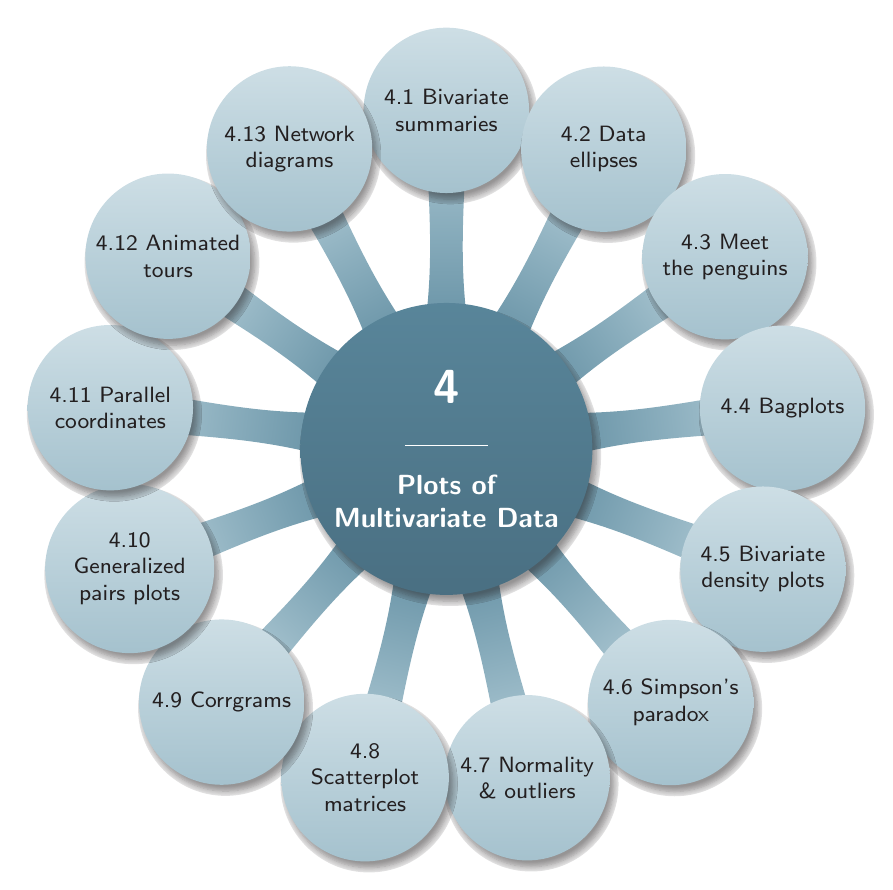
\begin{tikzpicture}[
  sat/.style={satbubble=partII, minimum size=2.1cm, text width=1.85cm,
              font=\sffamily\footnotesize}]
% connection bands (drawn first; the bubbles cover their ends)
\band{partII}{90}{4.3}
\band{partII}{62.3}{4.3}
\band{partII}{34.6}{4.3}
\band{partII}{6.9}{4.3}
\band{partII}{339.2}{4.3}
\band{partII}{311.5}{4.3}
\band{partII}{283.8}{4.3}
\band{partII}{256.1}{4.3}
\band{partII}{228.4}{4.3}
\band{partII}{200.7}{4.3}
\band{partII}{173}{4.3}
\band{partII}{145.3}{4.3}
\band{partII}{117.6}{4.3}
% bubbles
\node[rootbubble=partII, minimum size=3.4cm, text width=3.0cm]
  {\bubbletitle{4}{Plots of Multivariate Data}};
\node[sat] at (90:4.3) {4.1 Bivariate summaries};
\node[sat] at (62.3:4.3) {4.2 Data ellipses};
\node[sat] at (34.6:4.3) {4.3 Meet the penguins};
\node[sat] at (6.9:4.3) {4.4 Bagplots};
\node[sat] at (339.2:4.3) {4.5 Bivariate density plots};
\node[sat] at (311.5:4.3) {4.6 Simpson's paradox};
\node[sat] at (283.8:4.3) {4.7 Normality \& outliers};
\node[sat] at (256.1:4.3) {4.8 Scatterplot matrices};
\node[sat] at (228.4:4.3) {4.9 Corrgrams};
\node[sat] at (200.7:4.3) {4.10 Generalized pairs plots};
\node[sat] at (173:4.3) {4.11 Parallel coordinates};
\node[sat] at (145.3:4.3) {4.12 Animated tours};
\node[sat] at (117.6:4.3) {4.13 Network diagrams};
\end{tikzpicture}
\end{document}
